\documentclass[12pt, a4paper]{article}
\usepackage[utf8]{inputenc}
\usepackage[russian]{babel}
\usepackage[pdftex]{graphicx, color}
\usepackage{amsmath, amsfonts, amssymb, amsthm}
\usepackage[left=2cm,right=1.5cm,top=1.5cm,bottom=2cm]{geometry}
\usepackage{indentfirst}

\usepackage{setspace}
\onehalfspacing
\graphicspath{{pic/}}

\begin{document}

	\thispagestyle{empty}

	\begin{singlespace}
	\begin{titlepage}
		\begin{center}
			
\includegraphics[height = 3cm]{msu.png}

			{\scshape Московский государственный университет имени М.~В.~Ломоносова}\\
			Факультет вычислительной математики и кибернетики\\
			\centerline{\hfill\hrulefill\hrulefill\hrulefill\hrulefill\hfill}

			\vfill

			{\LARGE Отчет к восьмому заданию практикума на ЭВМ: \\ Коды БЧХ}

			\vspace{1cm}

		\end{center}

		\vfill
		\begin{flushright}
			Студент 317 группы:\\
				\textit{Оспанов А.М.}

			\vspace{5mm}

		\end{flushright}

		\vfill

		\begin{center}
		Москва, 2015
		\end{center}
	\end{titlepage}
	\end{singlespace}

	\tableofcontents


	\newpage
	\section{Введение}
		Данный отчет написан к восьмому заданию практикума на ЭВМ 317 группы. Тема задания: Коды БЧХ. Отчет написан студентом 317 группы -- Оспановым Аятом.

		В данной работе были реализованы модули gf.py и bch.py со всеми функциями. Были проведены исследования зависимости скорости БЧХ-кода от количества исправляемых кодом ошибок t для различных значений n и оценены доли правильно раскодированных сообщений, доли ошибочно раскодированных сообщений и доли отказов от декодирования для БЧХ-кода и проведено сравнение времени работы декодера Евклида и декодера PGZ.

		Код написан на языке Python с использованием библиотеки numpy.

	\newpage
	\section{Основная часть}
		\subsection{Скорость БЧХ-кода}
			Построим графики зависимости скорости БЧХ-кода r = k/n от количества исправляемых кодом ошибок t для различных значений n.

			\begin{center}
				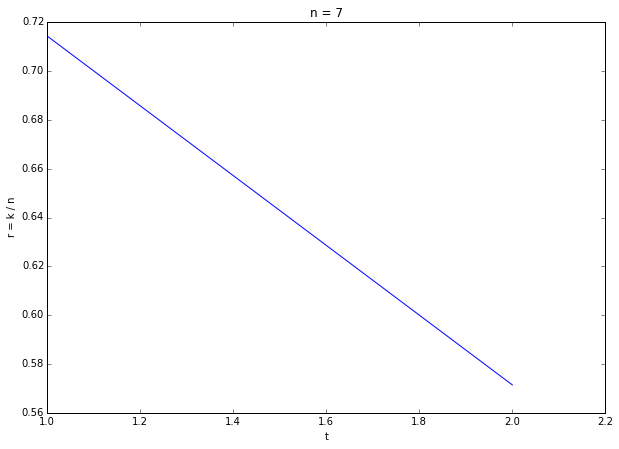
\includegraphics[width=8cm]{n7.png}
				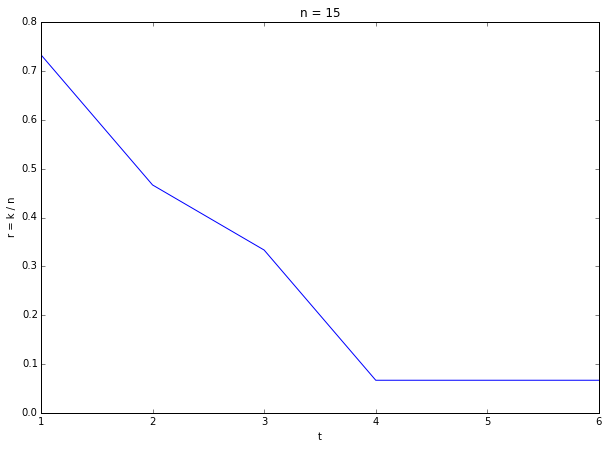
\includegraphics[width=7.9cm]{n15.png}
				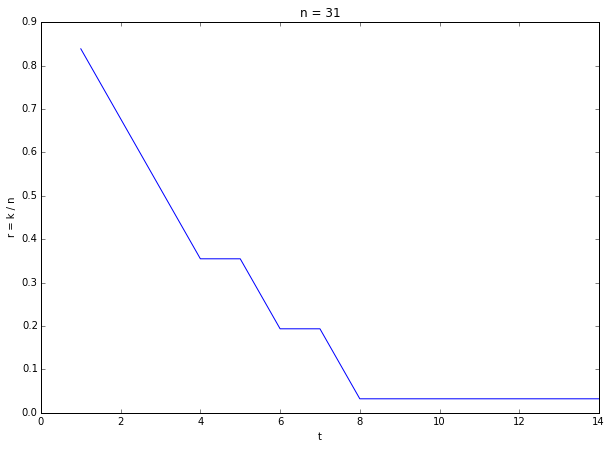
\includegraphics[width=7.9cm]{n31.png}
				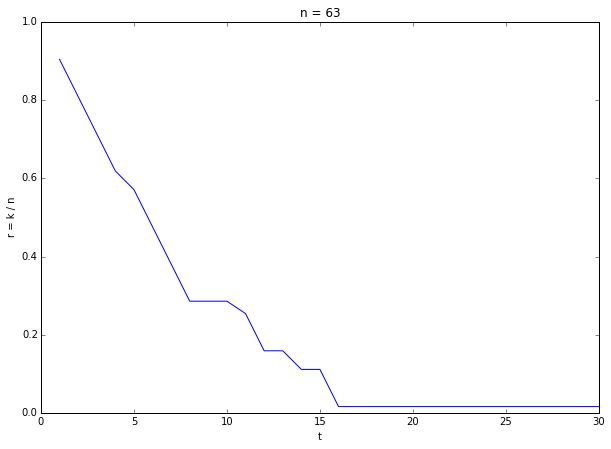
\includegraphics[width=7.9cm]{n63.png}
				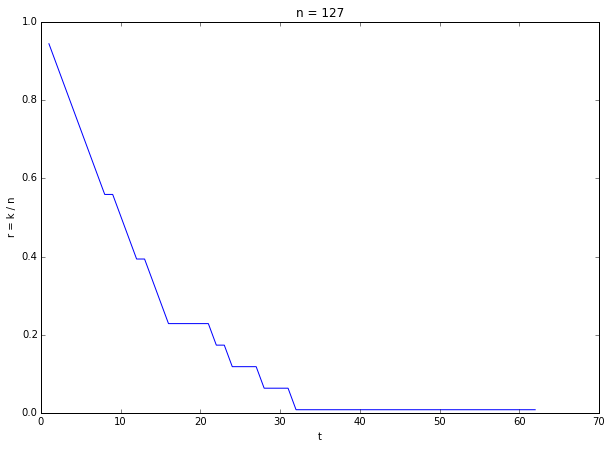
\includegraphics[width=7.9cm]{n127.png}
				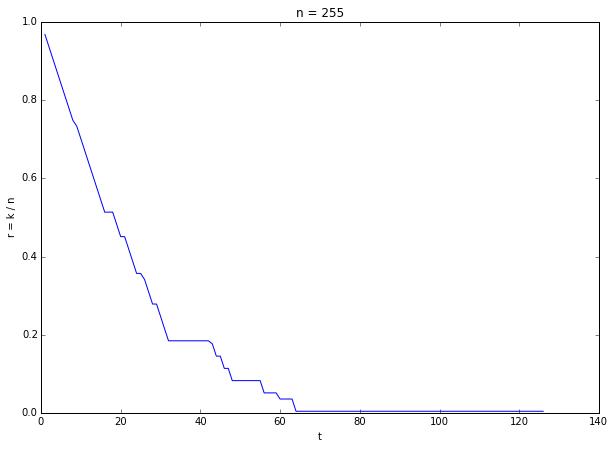
\includegraphics[width=7.9cm]{n255.png}
				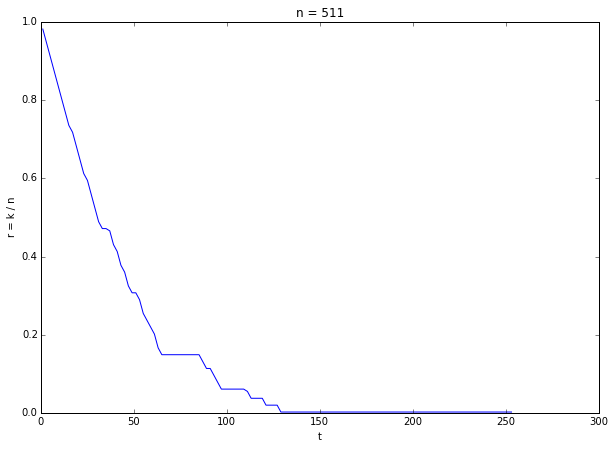
\includegraphics[width=7.9cm]{n511.png}
				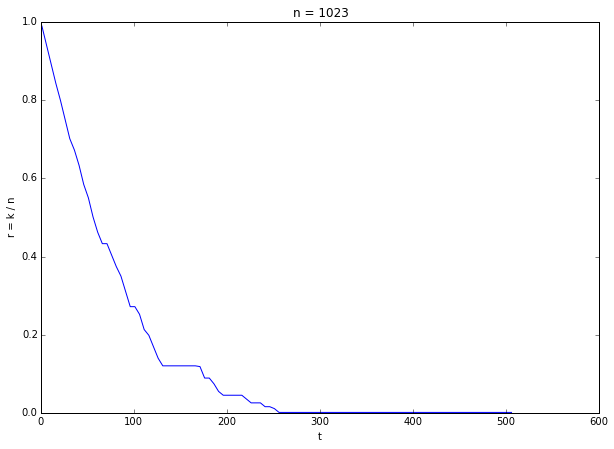
\includegraphics[width=7.9cm]{n1023.png}
				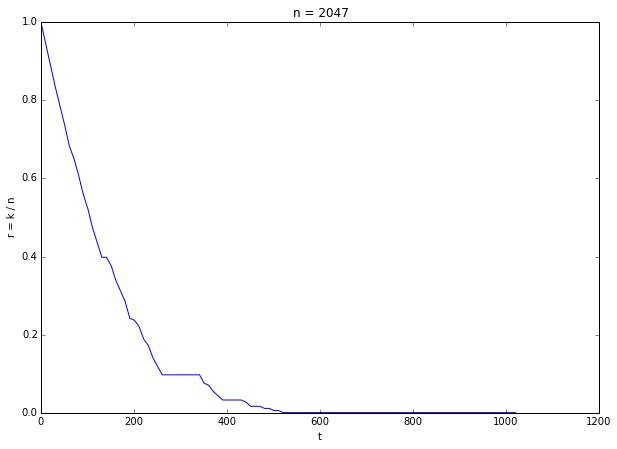
\includegraphics[width=7.9cm]{n2047.png}
				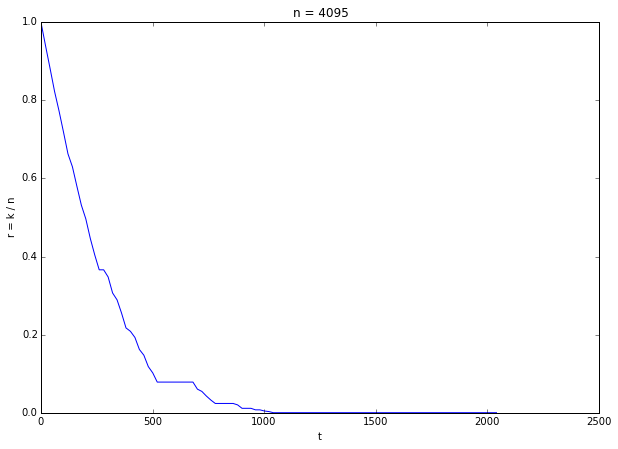
\includegraphics[width=7.9cm]{n4095.png}
			\end{center}

			Из графика видно, что при увеличении t, скорость БЧХ-кода будет снижаться экспоненциально.

			Значения t можно выбирать не больше, чем $\lfloor (n - 1) / 2 \rfloor $.

		\subsection{Пример БЧХ-кода, для которого истинное минимальное расстояние больше, чем величина 2t + 1}
			В качестве примера можно привести БЧХ-код, задаваемые следующими параметрами: $n = 15, t = 1, 2, 3, 4, 5, 6$. Для этих кодов, минимальными расстояниями будут: $l = 5, 8, 11, 15, 15, 15$. А значения $2t + 1 = 3, 5, 7, 9, 11, 13$


		\subsection{Сравнение двух методов декодирования по времени работы}
			Далее приведены графики зависимостей времени работы от t для декодера Евклида и декодера PGZ. Как видно из графиков, декодер Евклида работает за линейное время, а декодер PGZ работает за экспоненциальное.
			\begin{center}
				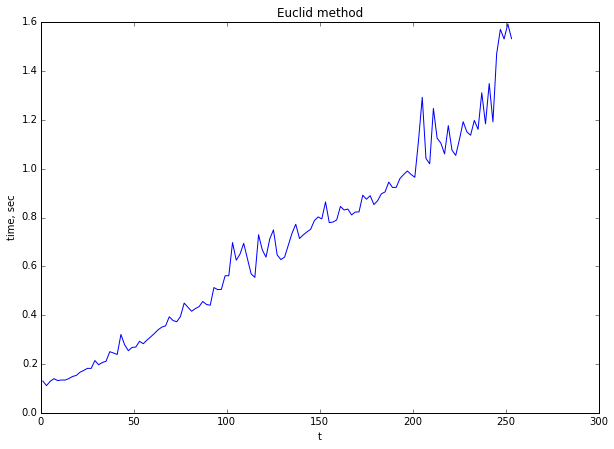
\includegraphics[width=8cm]{euclid.png}
				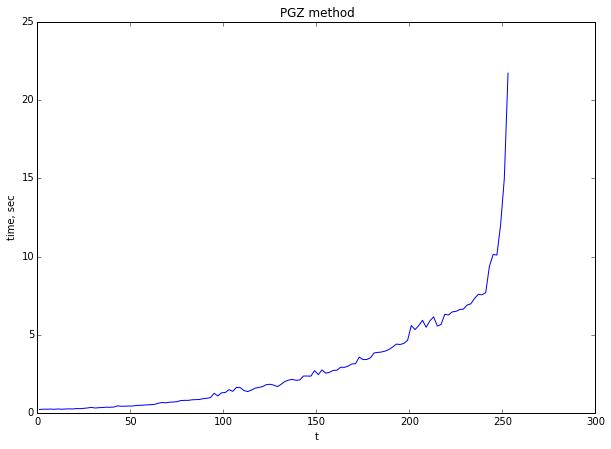
\includegraphics[width=8cm]{pgz.png}
			\end{center}

		\subsection{Оценка работы БЧХ-кода}
			В этом разделе было проведено статистическое испытание для оценки качества декодирования БЧХ-кода исправляющих t ошибок. Как видно из следующего графика, если допускаются ошибки в количестве меньшем, чем t, то доля правильно раскодированных сообщений почти 100\%, а доля ошибочно раскодированных сообщений и доля отказов минимальна и стремится к 0\%. Но если ошибок станет больше, чем t, то доля правильно раскодированных сообщений будет резко уменьшаться и станет 0\%, а доля отказов будет резко увеличиваться и станет 100\%. При этом, доля ошибок все равно минимальна и почти 0\%, что показывает, что БЧХ-код почти не допускает ошибок.
			\begin{center}
				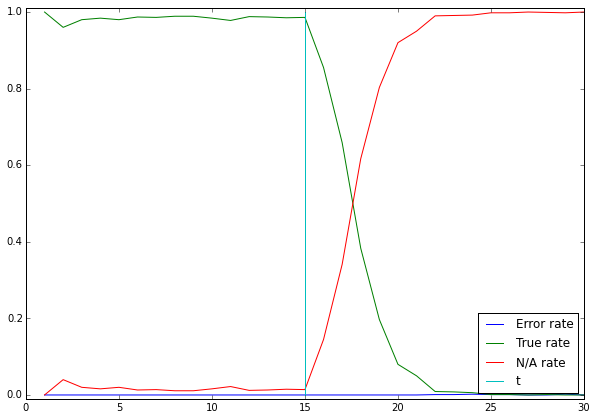
\includegraphics[width=12cm]{rates.png}
			\end{center}



	\newpage
	\section{Заключение}
		В результате исследовательской работы выяснилось, что БЧХ-код почти не допускает ошибочной раскодировки. Он либо правильно раскодирует, либо откажется от раскодирования. Также было выяснено, что скорость работы декодера Евклида больше, чем скорость работы декодера PGZ.

\end{document}
